\section{Skeletonization}

Skeletonization can be seen either as integral part of surface visualization techniques or as an separate preprocessing step. Actually both is true according to the observed methods as some surface visualization techniques compute the skeleton in an internal stage of the process. Here we focus on the preprocessing step.
Skeletonization here is actually a reduction of dimension on the segmentation data. We actually reduce the volumetric segmentation data or two dimensional surface data to a one dimensional graph structure. Nevertheless the graph itself is embedded in a 3D space.
The skeleton itself is a compact representation of 2D or 3D shapes that preserves many of the topological and size characteristics \cite{alexandru2002augmented}. Bium et al.~\cite{bium1964transformation} provides a common definition of the skeleton as the locus of centers of maximal discs (or spheres) contained in the original object.

There are actually three ways of generating skeletons and medial axes. The first one is \emph{morphological thinning} there the boundary of an object is peeled off layer by layer till those points remain which removal would cause topological change \cite{alexandru2002augmented}. As this is based on heuristics and is not based on the maximal discs approach this is the weakest of the skeletonization techniques, though the easiest one. The second is based on \emph{Voronoi diagrams} where the diagram represent the boundary's medial axis \cite{alexandru2002augmented}. While the most accurate one, this technique is also the most complex and expensive one. The third way is based on \emph{distance transforms} of oebject's boundaries \cite{alexandru2002augmented}. Here Sethian et al.~\cite{sethian1996fast} proposed the \emph{Fast Marching Method} (FFM) for evolution of boundaries in normal direction where the skeleton lies along the singularites. However the detection of those singularities is difficult and possibly unstable.

\begin{figure}[h]
	\centering
	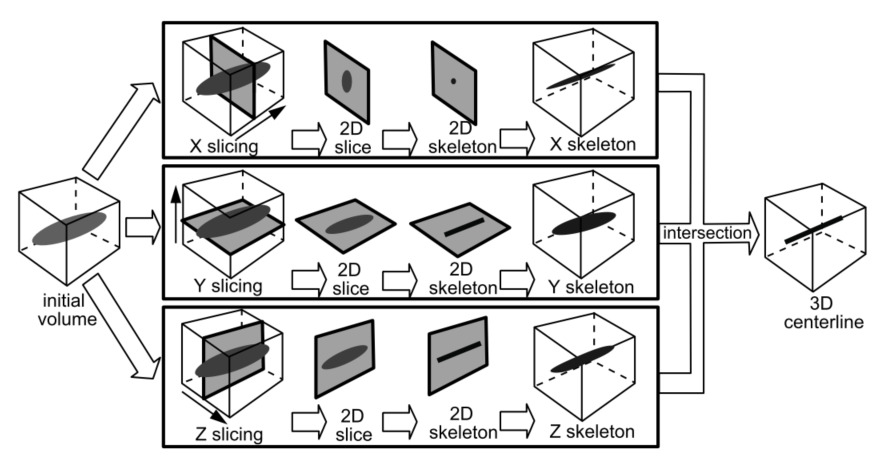
\includegraphics[width=0.4\textwidth]{./Images/CenterlineComputation.jpg} \\
	\caption{Centerline computation pipeline.}
	\cite{alexandru2002augmented}
	\label{fig:CenterlineComputation}
\end{figure} 

Telea et al.~\cite{alexandru2002augmented} augment the Fast Machring Method by computing the parametrized boundary location every pixel came from. The resulting prameter field is thresholded to produce the skeleton branches.
As his initial attemt focus on 2D problems he did an extension on 3D that utilize three distance transforms on the corresponding axis-parallel planes and intersect the resulting volumes to get a 3D centerline on the object as shown in figure \ref{fig:CenterlineComputation}.

\begin{figure}[h]
	\centering
	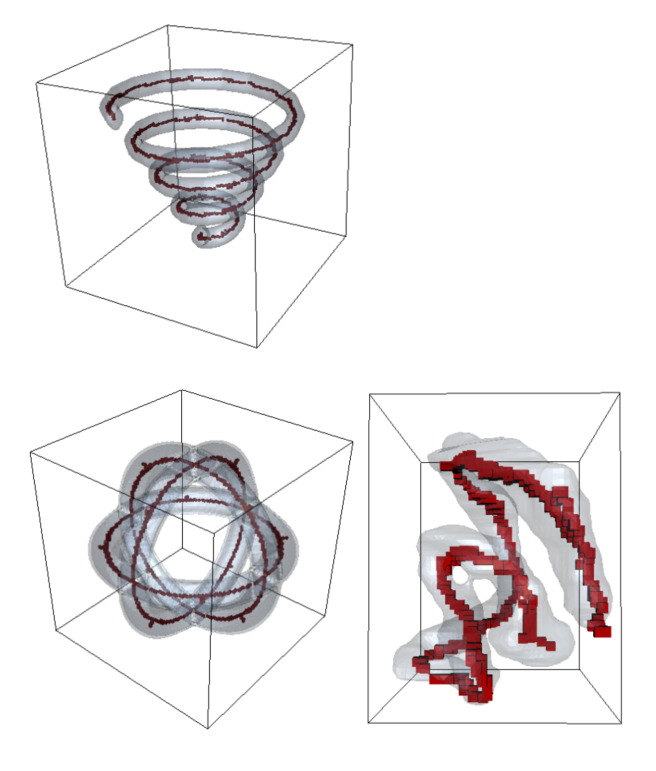
\includegraphics[width=0.33\textwidth]{./Images/ExampleCenterlines_II.jpg} \\
	\caption{Examples of 3D centerlines.}
	\cite{alexandru2002augmented}
	\label{fig:ExampleCenterlines_II}
\end{figure} 

As this approach do only respect the maximum distance from the boundary in the three orthogonal slice planes it is only an approximation. The real centerline would be at the location where centers of boundary-touching spheres are positioned. But for real world data the difference do not seem to be of big impact as shown in figure \ref{fig:ExampleCenterlines_II}. 

\begin{figure}[h]
	\centering
	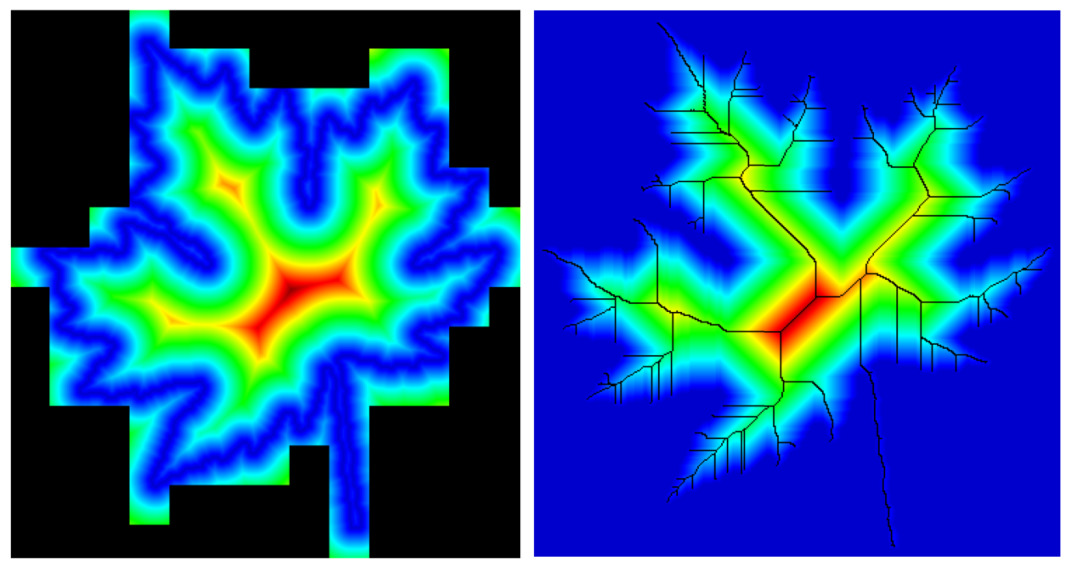
\includegraphics[width=0.45\textwidth]{./Images/LeafTilingAndDistanceTransform.jpg} \\
	\caption{Tiling and skeleton of a leaf.}
	\cite{strzodka2004generalized}
	\label{fig:LeafTilingAndDistanceTransform}
\end{figure} 

Strzodka et al.~\cite{strzodka2004generalized} further accelerates the generation of the 2D skeleton using graphics hardware. Based on the concept of \emph{footprint splatting} the combination of different spalts produces a weighted distance transform in real time. \emph{Distance splatting} uses OpenGL fragments to propagate signals in the \emph{feature distance transform} (FDT). The FDT follows the previously described concept that skeletons are defined as the set of centers of maximal balls contained in the boundary of the observed object. Tiling of the original object further speeds up the process. Results are pixel-level correct skeletons for all boundaries and thresholds, as shown in figure \ref{fig:LeafTilingAndDistanceTransform}.


% reduction of one dimension 